%%%%%%%%%%%%%%%%%%%%%%%%%%%%%%%%%%%%%%%%%
% Journal Article
% LaTeX Template
% Version 1.3 (9/9/13)
%
% This template has been downloaded from:
% http://www.LaTeXTemplates.com
%
% Original author:
% Frits Wenneker (http://www.howtotex.com)
%
% License:
% CC BY-NC-SA 3.0 (http://creativecommons.org/licenses/by-nc-sa/3.0/)
%
%%%%%%%%%%%%%%%%%%%%%%%%%%%%%%%%%%%%%%%%%

%----------------------------------------------------------------------------------------
%	PACKAGES AND OTHER DOCUMENT CONFIGURATIONS
%----------------------------------------------------------------------------------------

\documentclass[twoside]{article}

\usepackage{graphicx} % Package to include images
\usepackage{appendix}

\usepackage{amsmath}

\usepackage[sc]{mathpazo} % Use the Palatino font
\usepackage[T1]{fontenc} % Use 8-bit encoding that has 256 glyphs
\linespread{1.05} % Line spacing - Palatino needs more space between lines
\usepackage{microtype} % Slightly tweak font spacing for aesthetics

\usepackage{mathtools}
\DeclarePairedDelimiter\abs{\lvert}{\rvert}%

\usepackage[hmarginratio=1:1,top=32mm,columnsep=20pt]{geometry} % Document margins
\usepackage{multicol} % Used for the two-column layout of the document
\usepackage[hypcap=false,hang, small,labelfont=bf,up,textfont=it,up]{caption} % Custom captions under/above floats in tables or figures
\usepackage{booktabs} % Horizontal rules in tables
\usepackage{float} % Required for tables and figures in the multi-column environment - they need to be placed in specific locations with the [H] (e.g. \begin{table}[H])
\usepackage[hidelinks]{hyperref} % For hyperlinks in the PDF

\usepackage{lettrine} % The lettrine is the first enlarged letter at the beginning of the text
%\usepackage{paralist} % Used for the compactitem environment which makes bullet points with less space between them

\usepackage{abstract} % Allows abstract customization
\renewcommand{\abstractnamefont}{\normalfont\bfseries} % Set the "Abstract" text to bold
\renewcommand{\abstracttextfont}{\normalfont\small} % Set the abstract itself to small italic text

\usepackage{titlesec} % Allows customization of titles
\renewcommand\thesection{\Roman{section}} % Roman numerals for the sections
\renewcommand\thesubsection{\Roman{subsection}} % Roman numerals for subsections
\titleformat{\section}[block]{\large\scshape\centering}{\thesection.}{1em}{} % Change the look of the section titles
\titleformat{\subsection}[block]{\large}{\thesubsection.}{1em}{} % Change the look of the section titles
\usepackage{listings}
\usepackage{color}

\definecolor{Blue}{rgb}{0,0,0.5}
\definecolor{Green}{rgb}{0,0.75,0.0}
\definecolor{LightGray}{rgb}{0.6,0.6,0.6}
\definecolor{DarkGray}{rgb}{0.3,0.3,0.3}
\newcommand\matlabstyle{\lstset{language=Matlab,
   keywords={function,uint8,uint16,uint32,double,break,case,catch,continue,else,elseif,end,for,global,if,otherwise,persistent,return,switch,try,while},
   basicstyle=\ttfamily\footnotesize,
   breaklines=true,
   keywordstyle=\bfseries\color{Blue},
   commentstyle=\itshape\color{LightGray},
   stringstyle=\color{Green},
   numbers=left,
   numberstyle=\tiny\color{DarkGray},
   stepnumber=1,
   numbersep=10pt,
   backgroundcolor=\color{white},
   tabsize=2,
   showspaces=false,
   showstringspaces=false,
   captionpos=b}}


%Use command \code for code snippets
\newcommand{\code}[1]{\textnormal{\texttt{#1}}}

% Matlab environment
\lstnewenvironment{matlab}[1][]
{
\matlabstyle
\lstset{#1}
}
{}

% Matlab for external files
\newcommand\matlabexternal[2][]{{
\matlabstyle
\lstinputlisting[#1]{#2}}}

% Matlab for inline
\newcommand\matlabinline[1]{{\matlabstyle\lstinline!#1!}}
\usepackage{nonfloat}
\newcommand\myfigure[1]{%
\medskip\noindent\begin{minipage}{\columnwidth}
\centering%
#1%
%figure,caption, and label go here
\end{minipage}\medskip}

\usepackage{fancyhdr} % Headers and footers
\pagestyle{fancy} % All pages have headers and footers
\fancyhead{} % Blank out the default header
\fancyfoot{} % Blank out the default footer
%\fancyhead[C]{Running title $\bullet$ November 2012 $\bullet$ Vol. XXI, No. 1} % Custom header text
\fancyfoot[RO,LE]{\thepage} % Custom footer text

%----------------------------------------------------------------------------------------
%	TITLE SECTION
%----------------------------------------------------------------------------------------

\title{
   \vspace{-15mm}\fontsize{24pt}{10pt}\selectfont\textbf{Neural Networks III - Learning by gradient descent}
} % Article title

\author{
   \large
   \hspace{6mm}\textsc{Han Kruiger} \hspace{12mm} \textsc{Maarten Terpstra}\\[2mm] % Your name
   \normalsize University of Groningen \\ % Your institution
   \normalsize \href{mailto:j.f.kruiger@student.rug.nl}{j.f.kruiger@student.rug.nl} \hspace{5mm} \normalsize \href{mailto:m.l.terpstra@student.rug.nl}{m.l.terpstra@student.rug.nl} % Your email address
   \vspace{-5mm}
}
\date{}

%----------------------------------------------------------------------------------------

\begin{document}

\maketitle % Insert title

\thispagestyle{fancy} % All pages have headers and footers

%----------------------------------------------------------------------------------------
%	ABSTRACT
%----------------------------------------------------------------------------------------

\begin{abstract}
   \noindent In this report, learning by stochastic gradient descent will be explained, implemented and applied to a given dataset.
   The training cost function and test cost function will be shown as a function of learning time.
   We will experiment with the size of the training set.
   Also, the learning rate will be varied, and the consequences of this will be analyzed.
\end{abstract}

%----------------------------------------------------------------------------------------
%	ARTICLE CONTENTS
%----------------------------------------------------------------------------------------

\begin{multicols}{2} % Two-column layout throughout the main article text
\section{Introduction}
\label{sec:intro}
%!TEX root = report.tex
Gradient descent can be used to minimize the cost function of a simple feedforward neural network.
The feedforward network that we consider has two layers, and its real-valued output is given by:
\[
	\sigma(\pmb{\xi}) = 
	\tanh(\mathbf{w}_1\cdot \pmb{\xi}) + \tanh(\mathbf{w}_2\cdot \pmb{\xi})
\]
The training dataset is given as:
\[
\mathbb{D}_{train} =
	\left\{
		\pmb{\xi}^\mu, \tau(\pmb{\xi}^\mu)
	\right\}_{\mu=1}^{P}
\]
Likewise, the test dataset is given as:
\[
\mathbb{D}_{test} =
	\left\{
		\pmb{\xi}^\mu, \tau(\pmb{\xi}^\mu)
	\right\}_{\mu=1}^{Q}
\]
The training dataset comes with real-valued training labels \(\tau(\pmb{\xi}^\mu)\), so the training cost function is given by:
\[
	E_{train} = 
	\frac{1}{2P}
	\sum_{\mu=1}^P(\sigma(\pmb{\xi}^\mu) - \tau(\pmb{\xi}^\mu))^2
\]
Likewise, the test cost function is given by:
\[
	E_{test} = 
	\frac{1}{2Q}
	\sum_{\mu=1}^Q(\sigma(\pmb{\xi}^\mu) - \tau(\pmb{\xi}^\mu))^2
\]
In every learning step, a random \(\pmb{\xi}^\nu\) is chosen from the \(P\) training examples.
\(\pmb{\xi}^\nu\)'s contribution to the cost function is given by:
\[
	e^\nu = 
	\frac{1}{2}\left(
		\sigma(\pmb{\xi}^\nu) - \tau(\pmb{\xi}^\nu
	\right)^2
\]
The gradient descent update for the weight vectors \(\mathbf{w}_j\) with \(j \in \left\{1, 2\right\}\) is:
\[
	\mathbf{w}_j \leftarrow \mathbf{w}_j - \eta \nabla_{\mathbf{w}_j}e^\nu
\]
where \(\eta\) is the learning rate, and \(\nabla_{\mathbf{w}_j}\) denotes the gradient with respect to \(\mathbf{w}_j\).

\(\nabla_{\mathbf{w}_j}e^\nu\), that is the gradient of the contribution of a single example to the cost function with respect to \(\mathbf{w}_j\), is given by:
\begin{align*}
	\nabla_{\mathbf{w}_j}e^\nu
	&= \\
	\frac{1}{2} \nabla_{\mathbf{w}_j} \left( 
		\sigma(\pmb{\xi}^\nu) - \tau(\pmb{\xi}^\nu)
	\right)^2
	&= \\
	(\sigma(\pmb{\xi}^\nu) - \tau(\pmb{\xi}^\nu))
	\nabla_{\mathbf{w}_j}
	\sigma(\pmb{\xi}^\nu)
	&= \\
	(\sigma(\pmb{\xi}^\nu) - \tau(\pmb{\xi}^\nu))
	\nabla_{\mathbf{w}_j}
	\tanh(\mathbf{w}_j\cdot\pmb{\xi}^\nu)
	&= \\
	(\sigma(\pmb{\xi}^\nu) - \tau(\pmb{\xi}^\nu))
	(1 - \tanh^2(\mathbf{w}_j\cdot\pmb{\xi}^\nu))
	\nabla_{\mathbf{w}_j}
	\mathbf{w}_j\cdot\pmb{\xi}^\nu
	&= \\
	(\sigma(\pmb{\xi}^\nu) - \tau(\pmb{\xi}^\nu))
	(1 - \tanh^2(\mathbf{w}_j\cdot\pmb{\xi}^\nu))
	\pmb{\xi}^\nu
\end{align*}

Performing the gradient descent update for \(t_{max} \cdot P\) random examples, stochastically results in a descent of the cost functions.

\[\]

\section{Implementation}
\label{sec:implementation}
%!TEX root = report.tex
The implementation of gradient descent learning is fairly straightforward. 
The implementation of the cost function as described in equation~\ref{eq:costFunction} proved very easy and natural to implement in MATLAB.
An excerpt of our code can be found in appendices~\ref{app:training} and~\ref{app:step}.

For the determination of the generalization error in terms of quadratic deviations we have diverged from the assignment description. 
In the assignment \(E_{test}\) there is one single loop over the training patterns and the test patterns. 
However, we have split the training patterns and the test patterns into two separate matrices for clarity and simplicity. 
This does mean that we are performing two separate loops over two matrices to determine the value \(E_{test}\) as opposed to one loop.

\section{Results}
\label{sec:results}
%!TEX root = report.tex
Running the Min-Over algorithm on a student perceptron yields a few interesting results. We present several results we have found here and discuss them in section~\ref{sec:discussion}. 

In all cases the number of neurons was 20, the values of $\alpha = (0.1, 0.2, 0.3, \ldots 4.9, 5.0)$. The value of delta was $10^{-5}$ and the value of $\text{n}_{\text{max}} = 200$.

\myfigure{
	\includegraphics[width=\columnwidth]{learningcurve_100_innerloops.eps}%
	\figcaption{The learning curve of the student perceptron. It shows the generalization error against $\alpha$. This is the average of 100 trainings per $\alpha$-value}
	\label{fig:learningcurve}
}

Figure~\ref{fig:learningcurve} shows the learning curve of the perceptron. It shows the generalization error against the value of $\alpha$, thus the number patterns over the number of input neurons. 

The generalization error determines the probability that disagreement occurs between the teacher perceptron and the student perceptron. Figures~\ref{fig:generalizationerror_50}-\ref{fig:generalizationerror_150} show the generalization error as a function of time.
\myfigure{
	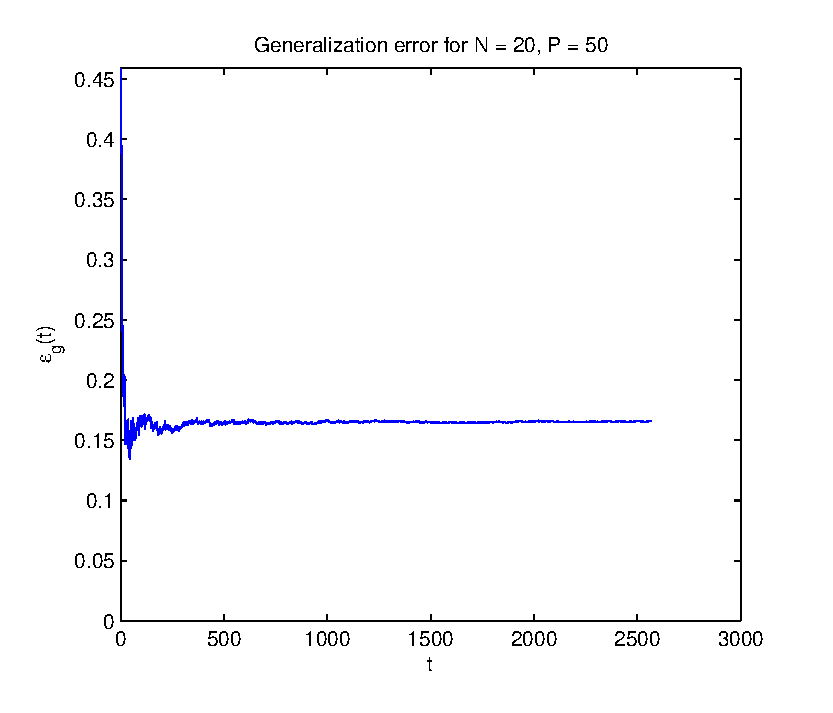
\includegraphics[width=\columnwidth]{generalizationerror_P_50.eps}%
	\figcaption{Generalization error for \(P=50\)}
	\label{fig:generalizationerror_50}
}
\myfigure{
	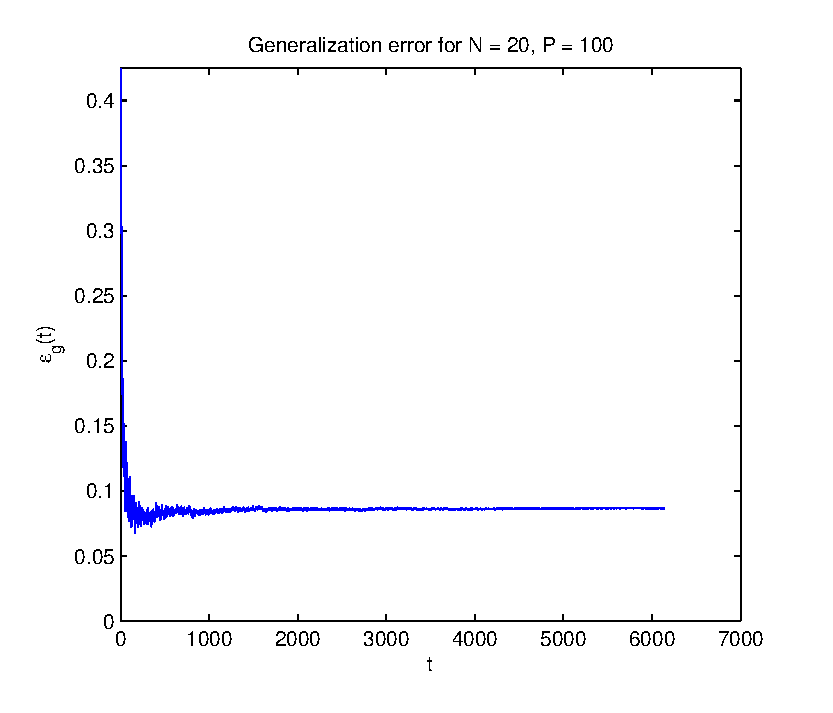
\includegraphics[width=\columnwidth]{generalizationerror_P_100.eps}%
	\figcaption{Generalization error for \(P=100\)}
	\label{fig:generalizationerror_100}
}
\myfigure{
	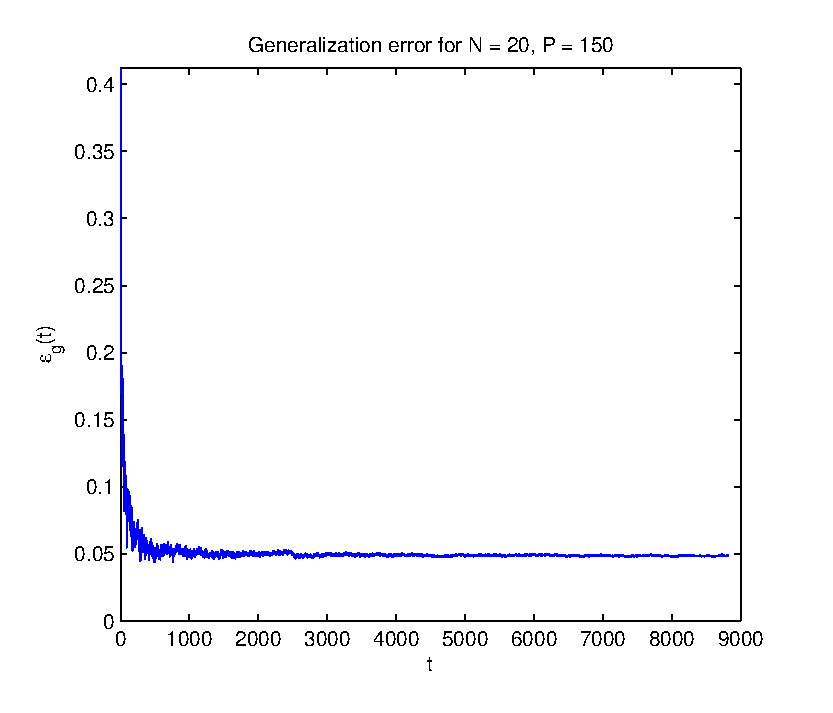
\includegraphics[width=\columnwidth]{generalizationerror_P_150.eps}%
	\figcaption{Generalization error for \(P=150\)}
	\label{fig:generalizationerror_150}
}
It can be seen in Figures~\ref{fig:generalizationerror_50}-\ref{fig:generalizationerror_150} that error converges relatively fast towards a certain value.

Moreover, the Min-Over algorithm has also been run on noisy data. There was 5\% noise added to the data. This means that approximately 5\% of the labels $S^{\mu}_R$ had a flipped sign as opposed to what the teacher perceptron trained. This should prove the robustness of the algorithm.
\myfigure{
	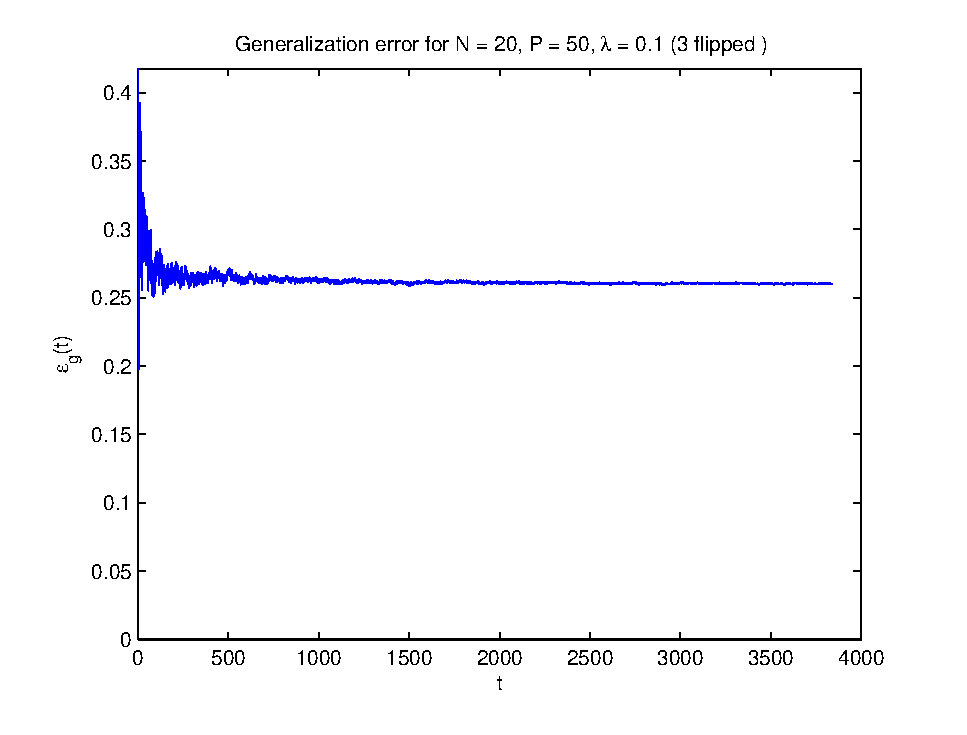
\includegraphics[width=\columnwidth]{generalizationerror_noisy.eps}%
	\figcaption{Generalization error for \(P=50\) with 5\% noise added.}
	\label{fig:generalizationerror_noisy}
}
Figure~\ref{fig:generalizationerror_noisy} shows the generalization error of the perceptron training with noisy data. In comparison with figure~\ref{fig:generalizationerror_50} it is visible that the system still converges to some value, but the convergence value is higher than with non-noisy training data. 

\myfigure{
	\includegraphics[width=\columnwidth]{learningcurve_noise.eps}%
	\figcaption{Learning curve of a student perceptron where 5\% noise is added to the data}
	\label{fig:noisecurve}
}
Figure~\ref{fig:noisecurve} shows the learning curve as figure~\ref{fig:learningcurve} does, but 5\% noise is added. They are somewhat similar but the curve of figure~\ref{fig:noisecurve} is less smooth as well as having an overall higher generalized error value.

\section{Discussion}
\label{sec:discussion}
%!TEX root = report.tex
One of the dangers of virtually every learning algorithm is overfitting. 
In this case, the trained model is too specific for the data and cannot correctly predict previously unforeseen observations because the generalization error increases as a result to a better fit to the training data. 
When the model is overfitted, it is highly unbiased towards the given data because it views all data as 'typical'.
As a result, the variance beyond the dataset is very large; the small fluctuations in the dataset are given too much meaning, causing it to incorrectly label data outside the trainingset.

One way to prevent overfitting is to perform the action of early stopping. 
This is a form of regularization to prevent overfitting. 
When early stopping is applied the number of iterations of algorithms as gradient descent is limited when it is detected that the machine is overfitting. 

Unfortunately, there are no formal methods to determine when to stop, as there are only ad-hoc manners to prevent overfitting. 
In our cases, we observe that overfitting can occur as soon as after 500 iterations (see figure~\ref{fig:overfitting}). 
Therefore, one way to perform early stopping for our dataset is to monitor the generalization error after 500 iterations.
If it increases as opposed to the previous iteration, the algorithm could decide to stop further training as it is starting to overfit.

\section{Conclusion}
\label{sec:conclusion}
%!TEX root = report.tex
In order to successfully implement gradient descent as a learning algorithm, one has to be careful in tuning its parameters. 
If the parameters are chosen incorrectly, the algorithm can quickly overfit (high variance) or underfit (high bias).
For our given dataset we have found that these parameters are most suited:
\begin{align*}
\eta &= 0.01 \\
P &= 4000 \\
t_{max} &= 100
\end{align*}

We have found that these parameters do indeed work correctly, as Figure~\ref{fig:costs_P4000} illustrates. 
The training error approaches a low value quite quickly and the test error approaches a constant value which is reasonably small (\(\sim 0.002\)).
We are quite pleased with these results.

\section{Workload division}
\label{sec:workload}
%!TEX root = report.tex
We did all the programming together.
Maarten focused mostly on reporting the implementation, results and discussion.
Han focused mostly on reporting the introduction, discussion and conclusion.

%----------------------------------------------------------------------------------------
%	REFERENCE LIST
%----------------------------------------------------------------------------------------
\bibliographystyle{ieeetr}
\bibliography{sources}

%----------------------------------------------------------------------------------------

\end{multicols}
\clearpage
\section*{Appendix}
\begin{appendices}
   \appendix
   \section{Gradient descent training}
   \label{app:training}
   \begin{matlab}
for t=1:t_max
    for i=1:P
        % Take a random example
        nu = randi(P);
        xi_nu = training_examples(:, nu);
        tau_nu = training_taus(nu);
        
        % Perform a gradient descent step using the random example
        [w_1, w_2] = gradient_descent_step(w_1, w_2, xi_nu, tau_nu, learning_rate);
    end
    
    % Store the cost functions at this time step
    training_cost = cost_function(training_examples, w_1, w_2, training_taus);
    training_costs(t) = training_cost;
    
    test_cost = cost_function(test_examples, w_1, w_2, test_taus);
    test_costs(t) = test_cost;
end
   \end{matlab}
   \section{Gradient descent step}
   \label{app:step}
   \matlabexternal{../gradient_descent_step.m}
\end{appendices}

\end{document}
